\begin{auf}
    380
\end{auf}
Der im $V,T$-Diagramm dargestellte Kreisprozess wird von einem idealen Gas ($\kappa=\frac{c_p}{c_V}=1.67$) zwischen den Temperaturen $T_1$ und $T_2=\frac{T_1}{2}$ durchlaufen.
\begin{enumerate}
    \item[a] Man übertrage die Darstellung in ein $p,V$-Diagramm.
    \item[b] Berechnen Sie die zu- und abgeführten Wärmen auf allen drei Teilwegen sowie die Kreisprozessarbeit für $T_1=500K$, $V_1=5l$ und $p_1=1MPa$.
    \item[c] Wie groß ist der thermische Wirkungsgrad $\eta_{th}$ einer nach diesem Kreisprozess arbeitenden Wärmekraftmaschine?
\end{enumerate}
\begin{figure}[h]
    \centering
    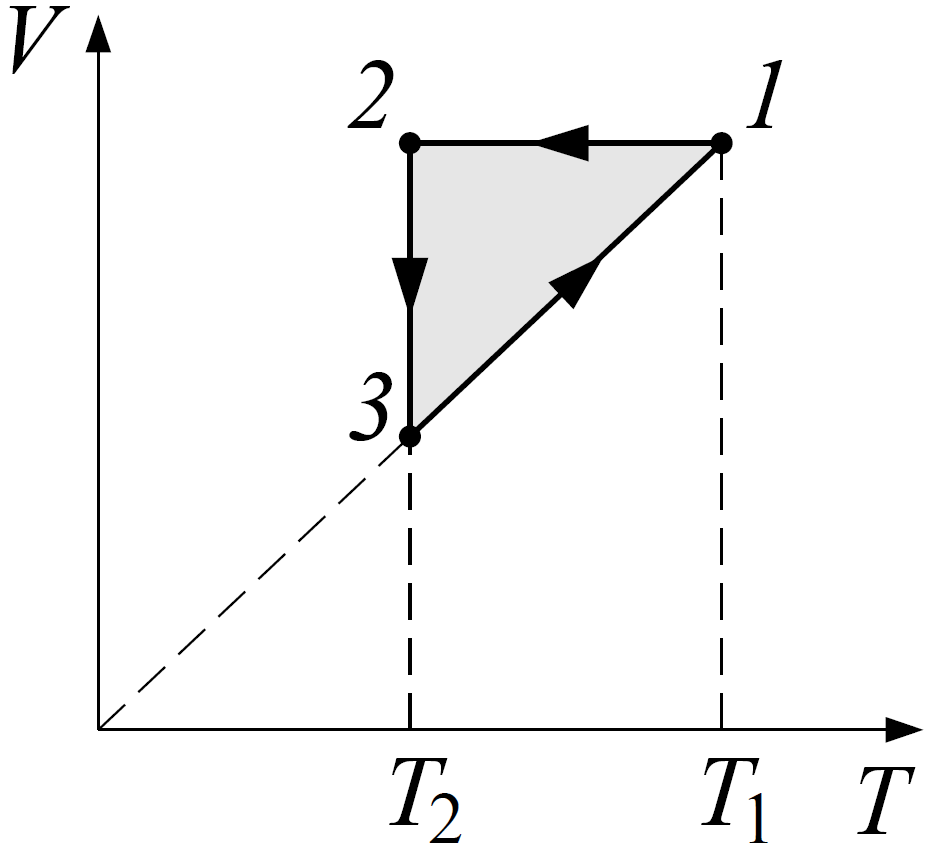
\includegraphics[height=5cm]{images/380_0.png}
    \caption{Versuchsaufbau Aufgabe 380}
\end{figure}